\chapter{Technology studies}

\textit{The technology studies covers the studies leading up to the design and implementation. The technology studies help give an overview of how to realise the power line communication bus by providing good knowledge into the theory needed.}

During the technology studies the procedure were:
\begin{enumerate}
\item Discover literature
\item Create overview
\item Read and understand
\item Experiment
\end{enumerate}
The studies below are partly based on previous knowledge from courses and experience and partly new knowledge and literature. The new literature can be found in appendix \fxfatal{reference!}.

\section{Protocol and communications}
\subsection{Communications}
The field of communication is very large, so to determine how to physically perform the communication in this system other methods were studied.\\
Communication systems use a lot of different ways of signaling data and it spans from frequency shift keying, phase shift keying, non-return to zero etc.
Commonly used for communication is level shifting (NRZ), this is known from many common communication protocols such as RS232, I$^2$C, SPI etc.\\
These physical protocol layers depend on synchronization either by including a clock or specifying a baudrate.\\
Another inspiration to the communcation layer of the project is the HART industrial protocol. HART is a protocol overlaying the 4-20mA standard. The HART protocol transmit a logic 1 with a 2200Hz frequency and a logic 0 with a 1200Hz frequency. This enables filtering to separate the analog data and the digital data. Often times the transmitters are loop powered meaning they are powered by the 4-20mA loop also similar to this project.
\subsection{Protocol}
To determine how the protocol should be structured, parallels to known communication protocols were made. The bus with multiple slaves/nodes has a lot of similarities physically with the I$^2$C protocol.\\
The I$^2$C protocol is a two wire system with multiple slaves, which responds to requests from the master. An I$^2$C transfer sequence is seen on the figure \ref{fig:i2cheader}. The figure originates from the I$^2$C protocol specification\cite{I2CInfo}.
\begin{figure}[H]
	\centering
	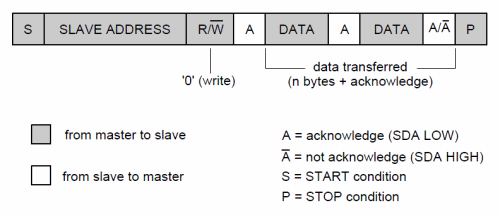
\includegraphics[width=.8\textwidth]{billeder/10technologystudies/7-bit-address-writing}
	\caption{I$^2$C protocol transfer sequence}
	\label{fig:i2cheader}
\end{figure}
The transfer sequence is initiated by a start sequence from the master, this alerts the slaves and they are now listening on the bus. The next step for the master is to transmit the address of the slave. An addressing system must be utilized because several slaves are connected to the bus. Lastly the master tells whether it is a read or write command. \\
The same principles are applied to the power line communication bus where an addressing system and start sequence is used.

Another known protocol is the modbus protocol\cite{Mbspec} which is a widely used industrial protocol. The modbus protocol has a start and addressing system, like I$^2$C. However after the address a function code is transmitted. This code is used to tell the slave exactly what to do. The modbus frame format is shown on figure \ref{fig:modbusframe}.
\begin{figure}[H]
	\centering
	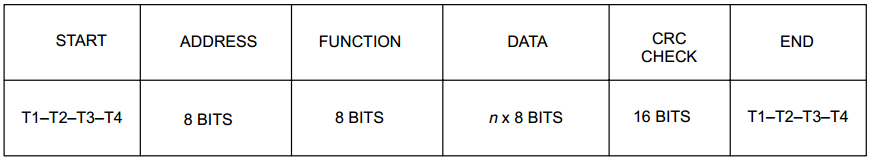
\includegraphics[width=.8\textwidth]{billeder/10technologystudies/modbusframe}
	\caption{Modbus frame/header}
	\label{fig:modbusframe}
\end{figure}
The function codes are standardized and covers a wide variety of uses, which covers all from simple request like, read discrete inputs, to diagnostic.
\section{Clock and data recovery}
Normally a data transmission consists of two elements, clock and data. That is not possible in this project and therefore the area of clock and data recovery was investigated.\\
Clock and data recovery is widely used in the field of data transmission. Especially in high bandwidth systems. Many of such systems use NRZ (Non-return to zero) line coding where in essence the clock is embedded in the data stream.\\
On figure \ref{fig:CDR} a conceptual block diagram of clock and data recovery is shown. From the recovered clock derived from the incoming data, the data is sampled.
\begin{figure}[hbpt]
	\centering
	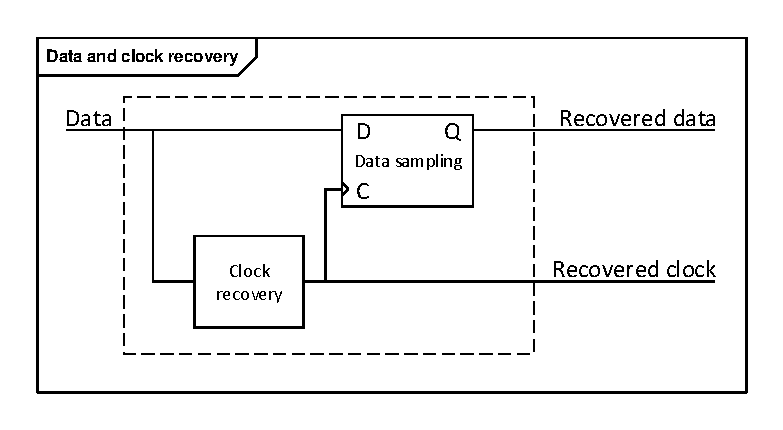
\includegraphics[width=.8\textwidth]{billeder/10technologystudies/CDR}
	\caption{Conceptual clock and data recovery block diagram}
	\label{fig:CDR}
\end{figure}
The clock recovery can be achieved by a variation of different solutions but commonly used is the phase locked loop(PLL). The following subsection will describe the basics of the PLL loop used in this project.
\subsection{The Phase-locked loop}
The PLL comes in a large variety of designs but they all have one common conceptual diagram. A PLL consists of a phase-detector, a filter and a voltage controlled oscillator(VCO). Optionally it can contain a clock divider to speed up the VCO clock. The structure of the conceptual PLL is shown in figure \ref{fig:conceptualpll}.
\begin{figure}[H]
	\centering
	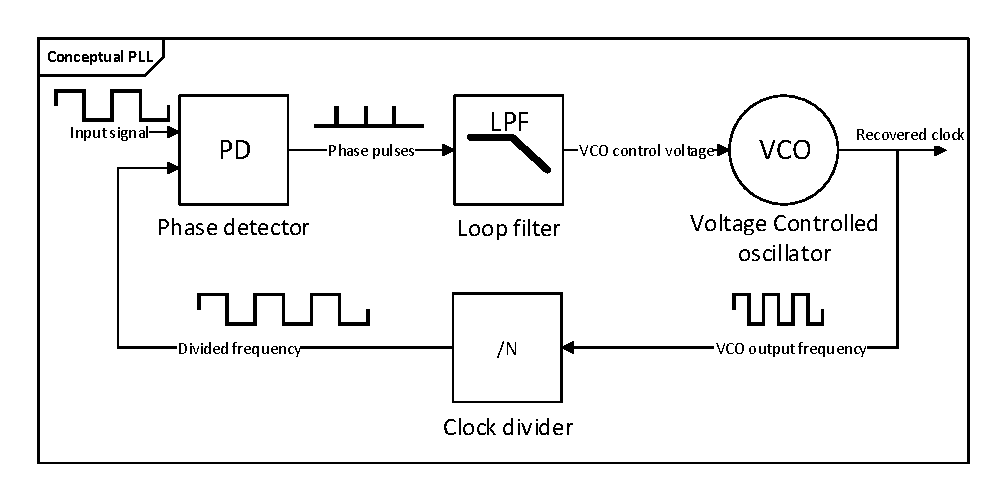
\includegraphics[width=.9\textwidth]{billeder/10technologystudies/conceptualpll}
	\caption{Conceptual PLL}
	\label{fig:conceptualpll}
\end{figure}
\subsubsection{Phase detector and loop filter}
The phase detector has two inputs. The input signal and the loop feedback signal. The phase detector compares the two input and produces a series of phase pulses depending on the phase difference of the two input signals. There is a variety of different phase detectors but two types are very common. They are named type 1 and type 2 phase detectors. Each type of detector has an impact on the loop.
\\ \textbf{Type 1:}\\
The type 1 phase detector is basically a XOR gate. 
\begin{figure}[H]
	\centering
	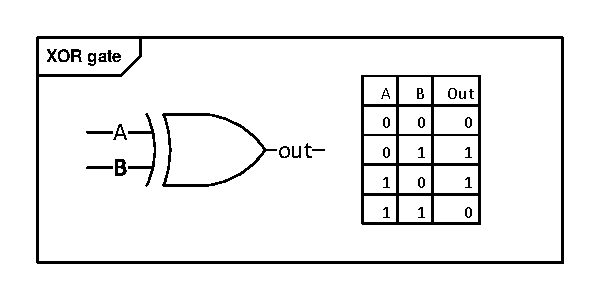
\includegraphics[width=.6\textwidth]{billeder/10technologystudies/XORgate}
	\caption{XOR gate}
	\label{fig:XOR}
\end{figure}
The XOR gate outputs a digital high when the two input signals are different from one another and a digital low when the two input signals are in the same state. Below on figure \ref{fig:pd1_waveforms} is shown the waveforms produced by a type 1 phase detector.
\begin{figure}[H]
	\centering
	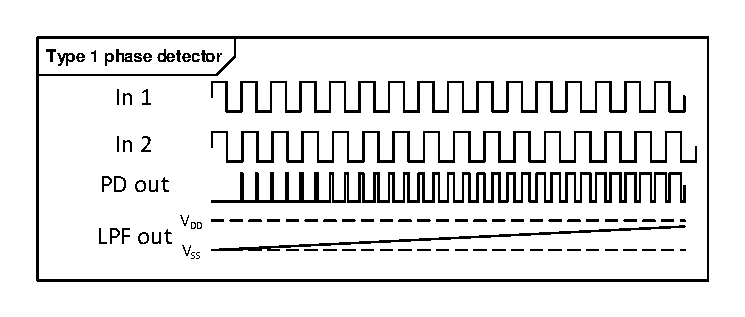
\includegraphics[width=.8\textwidth]{billeder/10technologystudies/PD1_waveforms}
	\caption{Phase detector type 1 waveforms}
	\label{fig:pd1_waveforms}
\end{figure}
The two input signals are different in frequency. And on the PD out line it is shown how this changes with regards to the two inputs.  The output of the low pass filter is used as an input to the VCO to either speed up the clock or slow it down.\\
When the PLL is locked onto the incoming frequency the LPF output will be $\frac{\text{V}_{\text{DD}}}{2}$. This effectively means that when the PLL locks onto the In 1 signal, the In 2 signal will be in exactly 90$^{\circ}$ deg phase.\\
\textbf{Type 2:}\\
The type 2 phase detector comprises of a phase comparator and a charge pump. The comparator is basically two D type flip-flops connected with and AND gate as seen on the figure \ref{fig:pd2_imp} below. The output from the phase comparator controls the charge pump to either charge or discharge the filter.
\begin{figure}[H]
	\centering
	\includegraphics[width=.7\textwidth]{billeder/10technologystudies/pd2_imp}
	\caption{Phase detector type 2 functional figure}
	\label{fig:pd2_imp}
\end{figure}
The advantage for the type 2 phase detector is the ability to detect a lead or a lag in frequency. Below on figure \ref{fig:pd2_waveform}, the waveform is illustrated for both leading and lagging. Depending on the amount of lead or lag the pump will be on/off for longer or shorter periods of time.
\begin{figure}[H]
	\centering
	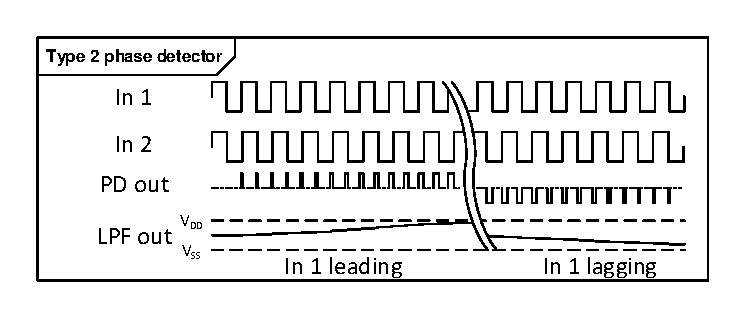
\includegraphics[width=1\textwidth]{billeder/10technologystudies/pd2_waveform}
	\caption{Phase detector type 2 waveforms}
	\label{fig:pd2_waveform}
\end{figure}
\subsubsection{Voltage controlled oscillator and Clock divider}
The voltage controlled oscillator serve to convert the voltage output of the LPF to an output frequency. The conceptual relationship between voltage input and frequency output is shown on figure \ref{fig:VCO_func}. The frequency increases as the voltage input increases. For the PLL to operate properly it is important that the VCO frequency output related to the voltage input is as linear as possible.The slope of this relationship must be positive at any times to ensure stability.
\begin{figure}[H]
	\centering
	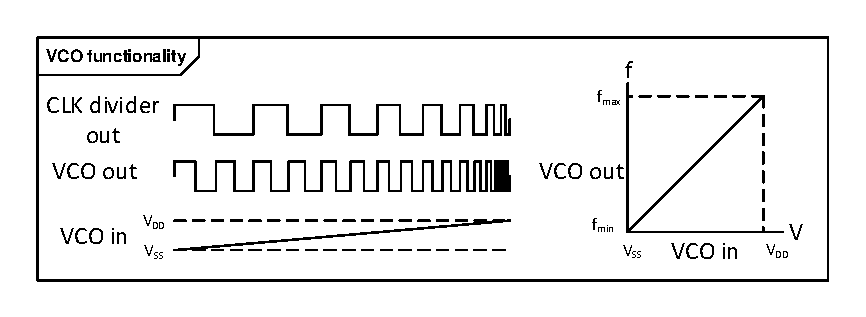
\includegraphics[width=1\textwidth]{billeder/10technologystudies/VCO_functionality}
	\caption{Voltage controlled oscillator functionality}
	\label{fig:VCO_func}
\end{figure}

\section{Outcome}
Based upon the technology studies several choices were made.\\
The daisy chain of sensor will be constructed as a current loop to power the sensors, much like the scheme used in the HART protocol. The main unit can then control the current to modulate communication to the sensors. The sensors will be addressable and will all have a unique address. They will respond to the function code scheme and the necessary codes will be determined in the architecture.\\
The communication will be based upon a NRZ scheme. This allows for simplicity as well as a lesser need for computational power to for example FSK. The NRZ scheme will enable for clock recovery using general purpose PPL's and this clock can be used to drive the sensor nodes. An extension to the NRZ line coding is manchester coding\cite{MC}. Although not covered above manchester coding ensures that the line is not low (or high) if a series of zeros (or ones) are transmitted. This helps to ensure a stable data sampling clock from the PLL. The manchester coding will follow the E. G. Thomas definitions\\
A minor part of the technology study was the study of the PIC24FJ µ-controller. The PIC24FJ was new to the group and some new knowledge had to be obtained. This was made easy by the PIC24 Tutorial on the engscope website \citep{Engscope}.



